% Created by tikzDevice version 0.12 on 2019-01-21 17:17:31
% !TEX encoding = UTF-8 Unicode
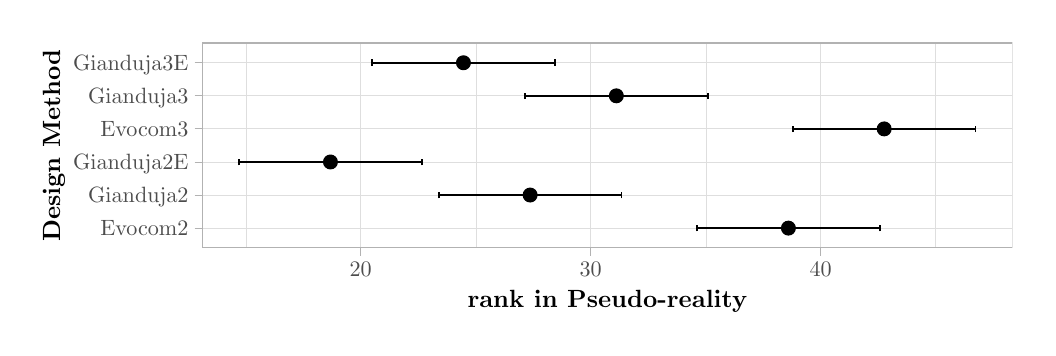
\begin{tikzpicture}[x=1pt,y=1pt]
\definecolor{fillColor}{RGB}{255,255,255}
\path[use as bounding box,fill=fillColor,fill opacity=0.00] (0,0) rectangle (361.35,108.41);
\begin{scope}
\path[clip] (  0.00,  0.00) rectangle (361.35,108.40);
\definecolor{drawColor}{RGB}{255,255,255}
\definecolor{fillColor}{RGB}{255,255,255}

\path[draw=drawColor,line width= 0.6pt,line join=round,line cap=round,fill=fillColor] (  0.00,  0.00) rectangle (361.35,108.40);
\end{scope}
\begin{scope}
\path[clip] ( 63.07, 28.81) rectangle (355.85,102.90);
\definecolor{fillColor}{RGB}{255,255,255}

\path[fill=fillColor] ( 63.07, 28.81) rectangle (355.85,102.90);
\definecolor{drawColor}{gray}{0.87}

\path[draw=drawColor,line width= 0.1pt,line join=round] ( 78.81, 28.81) --
	( 78.81,102.90);

\path[draw=drawColor,line width= 0.1pt,line join=round] (161.89, 28.81) --
	(161.89,102.90);

\path[draw=drawColor,line width= 0.1pt,line join=round] (244.98, 28.81) --
	(244.98,102.90);

\path[draw=drawColor,line width= 0.1pt,line join=round] (328.06, 28.81) --
	(328.06,102.90);

\path[draw=drawColor,line width= 0.3pt,line join=round] ( 63.07, 35.98) --
	(355.85, 35.98);

\path[draw=drawColor,line width= 0.3pt,line join=round] ( 63.07, 47.93) --
	(355.85, 47.93);

\path[draw=drawColor,line width= 0.3pt,line join=round] ( 63.07, 59.88) --
	(355.85, 59.88);

\path[draw=drawColor,line width= 0.3pt,line join=round] ( 63.07, 71.83) --
	(355.85, 71.83);

\path[draw=drawColor,line width= 0.3pt,line join=round] ( 63.07, 83.78) --
	(355.85, 83.78);

\path[draw=drawColor,line width= 0.3pt,line join=round] ( 63.07, 95.73) --
	(355.85, 95.73);

\path[draw=drawColor,line width= 0.3pt,line join=round] (120.35, 28.81) --
	(120.35,102.90);

\path[draw=drawColor,line width= 0.3pt,line join=round] (203.44, 28.81) --
	(203.44,102.90);

\path[draw=drawColor,line width= 0.3pt,line join=round] (286.52, 28.81) --
	(286.52,102.90);
\definecolor{drawColor}{RGB}{0,0,0}
\definecolor{fillColor}{RGB}{0,0,0}

\path[draw=drawColor,line width= 0.4pt,line join=round,line cap=round,fill=fillColor] (274.89, 35.98) circle (  2.50);

\path[draw=drawColor,line width= 0.4pt,line join=round,line cap=round,fill=fillColor] (181.56, 47.93) circle (  2.50);

\path[draw=drawColor,line width= 0.4pt,line join=round,line cap=round,fill=fillColor] (109.41, 59.88) circle (  2.50);

\path[draw=drawColor,line width= 0.4pt,line join=round,line cap=round,fill=fillColor] (309.50, 71.83) circle (  2.50);

\path[draw=drawColor,line width= 0.4pt,line join=round,line cap=round,fill=fillColor] (212.71, 83.78) circle (  2.50);

\path[draw=drawColor,line width= 0.4pt,line join=round,line cap=round,fill=fillColor] (157.46, 95.73) circle (  2.50);

\path[draw=drawColor,line width= 0.6pt,line join=round] (307.92, 34.78) --
	(307.92, 37.17);

\path[draw=drawColor,line width= 0.6pt,line join=round] (307.92, 35.98) --
	(241.85, 35.98);

\path[draw=drawColor,line width= 0.6pt,line join=round] (241.85, 34.78) --
	(241.85, 37.17);

\path[draw=drawColor,line width= 0.6pt,line join=round] (214.60, 46.74) --
	(214.60, 49.13);

\path[draw=drawColor,line width= 0.6pt,line join=round] (214.60, 47.93) --
	(148.52, 47.93);

\path[draw=drawColor,line width= 0.6pt,line join=round] (148.52, 46.74) --
	(148.52, 49.13);

\path[draw=drawColor,line width= 0.6pt,line join=round] (142.45, 58.69) --
	(142.45, 61.08);

\path[draw=drawColor,line width= 0.6pt,line join=round] (142.45, 59.88) --
	( 76.38, 59.88);

\path[draw=drawColor,line width= 0.6pt,line join=round] ( 76.38, 58.69) --
	( 76.38, 61.08);

\path[draw=drawColor,line width= 0.6pt,line join=round] (342.54, 70.64) --
	(342.54, 73.03);

\path[draw=drawColor,line width= 0.6pt,line join=round] (342.54, 71.83) --
	(276.46, 71.83);

\path[draw=drawColor,line width= 0.6pt,line join=round] (276.46, 70.64) --
	(276.46, 73.03);

\path[draw=drawColor,line width= 0.6pt,line join=round] (245.75, 82.59) --
	(245.75, 84.98);

\path[draw=drawColor,line width= 0.6pt,line join=round] (245.75, 83.78) --
	(179.67, 83.78);

\path[draw=drawColor,line width= 0.6pt,line join=round] (179.67, 82.59) --
	(179.67, 84.98);

\path[draw=drawColor,line width= 0.6pt,line join=round] (190.50, 94.54) --
	(190.50, 96.93);

\path[draw=drawColor,line width= 0.6pt,line join=round] (190.50, 95.73) --
	(124.42, 95.73);

\path[draw=drawColor,line width= 0.6pt,line join=round] (124.42, 94.54) --
	(124.42, 96.93);
\definecolor{drawColor}{gray}{0.70}

\path[draw=drawColor,line width= 0.6pt,line join=round,line cap=round] ( 63.07, 28.81) rectangle (355.85,102.90);
\end{scope}
\begin{scope}
\path[clip] (  0.00,  0.00) rectangle (361.35,108.41);
\definecolor{drawColor}{gray}{0.30}

\node[text=drawColor,anchor=base east,inner sep=0pt, outer sep=0pt, scale=  0.80] at ( 58.12, 33.22) {Evocom2};

\node[text=drawColor,anchor=base east,inner sep=0pt, outer sep=0pt, scale=  0.80] at ( 58.12, 45.18) {Gianduja2};

\node[text=drawColor,anchor=base east,inner sep=0pt, outer sep=0pt, scale=  0.80] at ( 58.12, 57.13) {Gianduja2E};

\node[text=drawColor,anchor=base east,inner sep=0pt, outer sep=0pt, scale=  0.80] at ( 58.12, 69.08) {Evocom3};

\node[text=drawColor,anchor=base east,inner sep=0pt, outer sep=0pt, scale=  0.80] at ( 58.12, 81.03) {Gianduja3};

\node[text=drawColor,anchor=base east,inner sep=0pt, outer sep=0pt, scale=  0.80] at ( 58.12, 92.98) {Gianduja3E};
\end{scope}
\begin{scope}
\path[clip] (  0.00,  0.00) rectangle (361.35,108.41);
\definecolor{drawColor}{gray}{0.70}

\path[draw=drawColor,line width= 0.3pt,line join=round] ( 60.32, 35.98) --
	( 63.07, 35.98);

\path[draw=drawColor,line width= 0.3pt,line join=round] ( 60.32, 47.93) --
	( 63.07, 47.93);

\path[draw=drawColor,line width= 0.3pt,line join=round] ( 60.32, 59.88) --
	( 63.07, 59.88);

\path[draw=drawColor,line width= 0.3pt,line join=round] ( 60.32, 71.83) --
	( 63.07, 71.83);

\path[draw=drawColor,line width= 0.3pt,line join=round] ( 60.32, 83.78) --
	( 63.07, 83.78);

\path[draw=drawColor,line width= 0.3pt,line join=round] ( 60.32, 95.73) --
	( 63.07, 95.73);
\end{scope}
\begin{scope}
\path[clip] (  0.00,  0.00) rectangle (361.35,108.41);
\definecolor{drawColor}{gray}{0.70}

\path[draw=drawColor,line width= 0.3pt,line join=round] (120.35, 26.06) --
	(120.35, 28.81);

\path[draw=drawColor,line width= 0.3pt,line join=round] (203.44, 26.06) --
	(203.44, 28.81);

\path[draw=drawColor,line width= 0.3pt,line join=round] (286.52, 26.06) --
	(286.52, 28.81);
\end{scope}
\begin{scope}
\path[clip] (  0.00,  0.00) rectangle (361.35,108.41);
\definecolor{drawColor}{gray}{0.30}

\node[text=drawColor,anchor=base,inner sep=0pt, outer sep=0pt, scale=  0.80] at (120.35, 18.35) {20};

\node[text=drawColor,anchor=base,inner sep=0pt, outer sep=0pt, scale=  0.80] at (203.44, 18.35) {30};

\node[text=drawColor,anchor=base,inner sep=0pt, outer sep=0pt, scale=  0.80] at (286.52, 18.35) {40};
\end{scope}
\begin{scope}
\path[clip] (  0.00,  0.00) rectangle (361.35,108.41);
\definecolor{drawColor}{RGB}{0,0,0}

\node[text=drawColor,anchor=base,inner sep=0pt, outer sep=0pt, scale=  0.90] at (209.46,  7.44) {\bfseries rank in Pseudo-reality};
\end{scope}
\begin{scope}
\path[clip] (  0.00,  0.00) rectangle (361.35,108.41);
\definecolor{drawColor}{RGB}{0,0,0}

\node[text=drawColor,rotate= 90.00,anchor=base,inner sep=0pt, outer sep=0pt, scale=  0.90] at ( 11.71, 65.86) {\bfseries Design Method};
\end{scope}
\end{tikzpicture}
